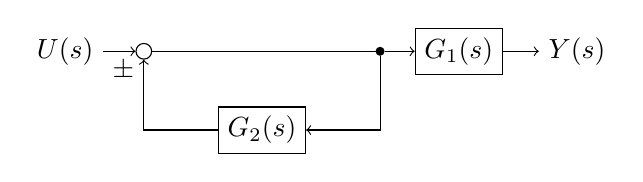
\begin{tikzpicture}
  \node (in) at (0,2) []{$U(s)$};
  \node (sum) at (1,2) [circle,draw,inner sep=2]{};
  \node (G1) at (5,2) [draw]{$G_1(s)$};
  \node (G2) at (2.5,1) [draw]{$G_2(s)$};
  \node (dot) at (4,2) [draw,circle,inner sep=1,fill]{};
  \node (out) at (6.5,2) []{$Y(s)$};

  \node (feedback) at (sum) [below left] {$\pm$};

  \draw[->] (in) -- (sum);
  \draw (sum) --  (dot);
  \draw[->] (dot) --  (G1);
  \draw[->](G1) -- (out);

  \draw[->] (dot) |-(G2);
  \draw[->] (G2) -| (sum);

\end{tikzpicture}
